% source: http://stackoverflow.com/a/4905034
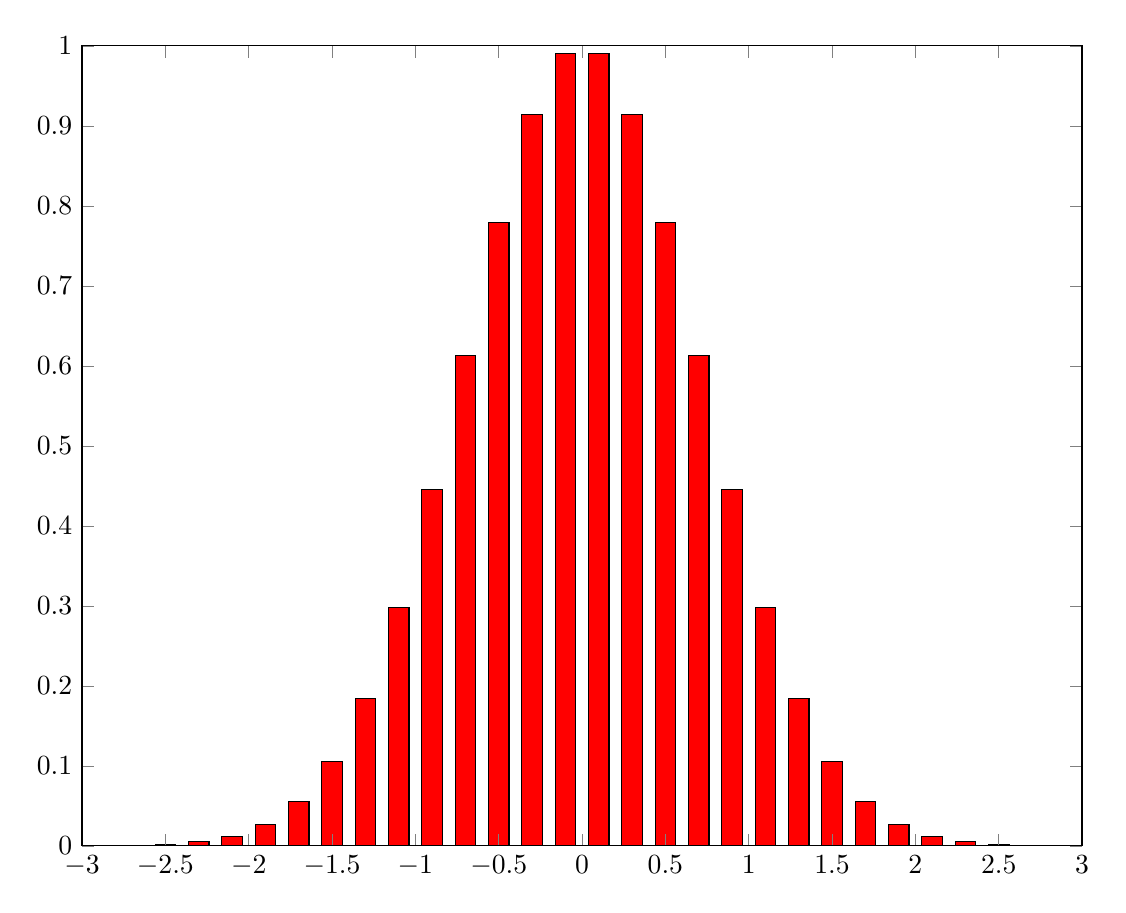
\begin{tikzpicture}[font=\sffamily]
    \begin{axis}[%
            scale only axis,
            width=5in,
            height=4in,
            xmin=-3, xmax=3,
            ymin=0, ymax=1,
        axis on top]
        \addplot[
            ybar,
            bar width=0.102874in,
            bar shift=0in,
            fill=red,
        draw=black]
        plot coordinates{
            (-2.9,0.00022263) (-2.7,0.000682328) (-2.5,0.00193045) (-2.3,0.00504176)
            (-2.1,0.0121552) (-1.9,0.0270518) (-1.7,0.0555762) (-1.5,0.105399)
            (-1.3,0.18452) (-1.1,0.298197) (-0.9,0.444858) (-0.7,0.612626)
            (-0.5,0.778801) (-0.3,0.913931) (-0.1,0.99005) (0.1,0.99005)
            (0.3,0.913931) (0.5,0.778801) (0.7,0.612626) (0.9,0.444858)
            (1.1,0.298197) (1.3,0.18452) (1.5,0.105399) (1.7,0.0555762)
            (1.9,0.0270518) (2.1,0.0121552) (2.3,0.00504176) (2.5,0.00193045)
            (2.7,0.000682328) (2.9,0.00022263)
        };
    \end{axis}
\end{tikzpicture}
